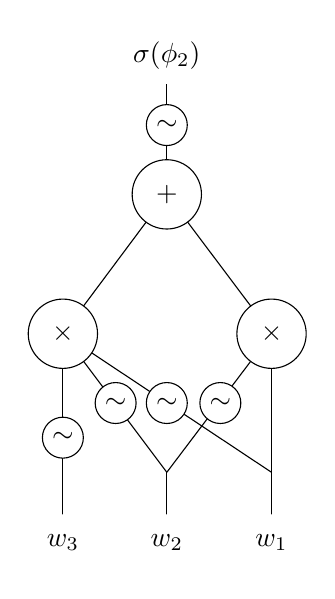
\begin{tikzpicture}
\definecolor{fillcolor}{RGB}{255,255,255}
\definecolor{highcolor}{RGB}{0,0,0}
\definecolor{lowcolor}{RGB}{0,0,0}
\definecolor{neutralcolor}{RGB}{0,0,0}
\definecolor{pathcolor}{RGB}{0,0,0}
\definecolor{background}{RGB}{225,225,225}
\draw (1.76,6.53) [thin,neutralcolor] -- (1.76,4.77);
\draw (1.76,4.77) [thin,neutralcolor] -- (0.44,3.00);
\draw (1.76,4.77) [thin,neutralcolor] -- (3.09,3.00);
\draw (0.44,3.00) [thin,neutralcolor] -- (3.09,1.24);
\draw (0.44,3.00) [thin,neutralcolor] -- (0.44,0.35);
\draw (0.44,3.00) [thin,neutralcolor] -- (1.76,1.24);
\draw (3.09,3.00) [thin,neutralcolor] -- (3.09,1.24);
\draw (3.09,3.00) [thin,neutralcolor] -- (1.76,1.24);
\draw (3.09,1.24) [thin,neutralcolor] -- (3.09,0.35);
\draw (1.76,1.24) [thin,neutralcolor] -- (1.76,0.35);
\draw [thin,fill=fillcolor,draw=fillcolor] (1.76,6.53) circle [radius=0.35];
\node at (1.76,6.53) {$\sigma(\phi_2)$};
\draw [thin,fill=fillcolor,draw=neutralcolor] (1.76,4.77) circle [radius=0.44];
\node at (1.76,4.77) {$+$};
\draw [thin,fill=fillcolor,draw=neutralcolor] (0.44,3.00) circle [radius=0.44];
\node at (0.44,3.00) {$\times$};
\draw [thin,fill=fillcolor,draw=neutralcolor] (3.09,3.00) circle [radius=0.44];
\node at (3.09,3.00) {$\times$};
\draw [thin,fill=neutralcolor,draw=neutralcolor] (3.09,1.24) circle [radius=0.00];
\node at (3.09,1.24) {};
\draw [thin,fill=neutralcolor,draw=neutralcolor] (1.76,1.24) circle [radius=0.00];
\node at (1.76,1.24) {};
\draw [thin,fill=fillcolor,draw=fillcolor] (3.09,0.35) circle [radius=0.35];
\node at (3.09,0.35) {$w_1$};
\draw [thin,fill=fillcolor,draw=fillcolor] (1.76,0.35) circle [radius=0.35];
\node at (1.76,0.35) {$w_2$};
\draw [thin,fill=fillcolor,draw=fillcolor] (0.44,0.35) circle [radius=0.35];
\node at (0.44,0.35) {$w_3$};
\draw [thin,fill=fillcolor,draw=neutralcolor] (1.76,5.65) circle [radius=0.26];
\node at (1.76,5.65) {$\sim$};
\draw [thin,fill=fillcolor,draw=neutralcolor] (1.76,2.12) circle [radius=0.26];
\node at (1.76,2.12) {$\sim$};
\draw [thin,fill=fillcolor,draw=neutralcolor] (1.11,2.12) circle [radius=0.26];
\node at (1.11,2.12) {$\sim$};
\draw [thin,fill=fillcolor,draw=neutralcolor] (2.44,2.12) circle [radius=0.26];
\node at (2.44,2.12) {$\sim$};
\draw [thin,fill=fillcolor,draw=neutralcolor] (0.44,1.68) circle [radius=0.26];
\node at (0.44,1.68) {$\sim$};
\end{tikzpicture}%%
